\input{$UNI_DIR/msc/tex/HWSetup}
\input{$UNI_DIR/msc/tex/EngBindings}

%
% Homework Details
%   - Title
%   - Subtitle
%   - Due date
%   - Due time
%   - Course
%   - Section/Time
%   - Instructor
%   - Author
%

\newcommand{\hmwkTitle}{HW01}
\newcommand{\hmwkSubTitle}{Orbits and 2BP}
\newcommand{\hmwkDueDate}{September 25th. 2025}
\newcommand{\hmwkDueTime}{09:30 AM}
\newcommand{\hmwkClass}{ENAE 441 - 0101}
\newcommand{\hmwkClassTime}{09:30 AM}
\newcommand{\hmwkClassInstructor}{Dr. Martin}
\newcommand{\hmwkAuthorName}{\textbf{Vai Srivastava}}
\newcommand{\hmwkCompletionDate}{\today}

\begin{document}

\maketitle

\pagebreak

\begin{hwkProblem}{1}{The Eccentricity Vector} \label{hwk:p01}

	\begin{enumerate}
		\item \label{hwk:p01a} Use the definition of the eccentricity vector \( \vecb{e} \) to prove that the total energy of the system, \[ \epsilon = \frac{\vecb{v} \cdot \vecb{v}}{2} - \frac{\mu}{r} \] is equal to \[ \epsilon = - \frac{\mu}{2 a} .\]
		\item \label{hwk:p01b} Use the expression \[ \epsilon = \frac{\vecb{v} \cdot \vecb{v}}{2} - \frac{\mu}{r} \] to prove that \[ \drv{\epsilon}{t} = 0 .\]
	\end{enumerate}

	\hwkSol{} \label{hwk:s01}

	\hwkPart{} \label{hwk:s01a}

	\begin{align*}
		\vecb{v} \cdot \vecb{v}           & = |\vecb{v}|^{2} = v^{2}                                                                       \\
		\vecb{v}                          & = \dot{\vecb{r}}                                                                               \\
		|\vecb{h}|                        & = h                                                                                            \\
		\vecb{e}                          & = \frac{1}{\mu} \left(\dot{\vecb{r}} \times \vecb{h} - \mu \frac{\vecb{r}}{|\vecb{r}|} \right) \\
		\dot{\vecb{r}} \times \vecb{h}    & = v h \hat{r}                                                                                  \\
		- \mu \frac{\vecb{r}}{|\vecb{r}|} & = - \mu \hat{r}                                                                                \\
		\implies \vecb{e}                 & = \left(\frac{v h}{\mu} - 1\right) \hat{r}                                                     \\
		\text{at periapsis:}              & \,                                                                                             \\
		r_{p} v_{p}                       & = h                                                                                            \\
		r_{p}                             & = a \left(1 - e\right)                                                                         \\
		\implies a                        & = \frac{r}{1-e}                                                                                \\
		\vecb{e}                          & = \left(\frac{r v^{2}}{\mu} - 1\right) \hat{r}                                                 \\
		\implies v^{2}                    & = \frac{\left(e + 1\right)\mu}{r}                                                              \\
		\epsilon                          & = \frac{v^{2}}{2} - \frac{\mu}{r}                                                              \\
		\,                                & = \frac{v^{2}}{1} - \frac{v^{2}}{e + 1}                                                        \\
		\,                                & = \frac{\left(e + 1\right) \mu}{2 r} - \frac{\mu}{r}                                           \\
		\,                                & = \frac{\left(e + 1\right)\mu - 2 \mu}{2 r}                                                    \\
		\,                                & = - \mu \frac{1 - e}{2 r}                                                                      \\
		\,                                & = - \frac{\mu}{2} \cancelto{\frac{1}{a}}{\left(\frac{1 - e}{r}\right)}                         \\
		\implies \epsilon                 & = - \frac{\mu}{2 a}
		.\end{align*}

	\hwkPart{} \label{hwk:s01b}

	\begin{align*}
		\epsilon                   & = \frac{\vecb{v} - \vecb{v}}{2} - \frac{\mu}{r}                                                 \\
		\,                         & = \frac{\dot{\vecb{r}} \cdotp \dot{\vecb{r}}}{2} - \frac{\mu}{r}                                \\
		\,                         & = \frac{\left(\dot{r}\right)^{2}}{2} - \frac{\mu}{r}                                            \\
		\drv{\epsilon}{t}          & = \frac{2 \dot{r} \ddot{r}}{2} + \frac{\mu \dot{r}}{r^{2}}                                      \\
		\,                         & = \dot{r} \left(\ddot{r} + \cancelto{- \ddot{r}}{\left(\frac{\mu}{r^{2}}\right)} \qquad \right) \\
		\,                         & = \dot{r} \, \cancelto{0}{\left(\ddot{r} - \ddot{r}\right)}                                     \\
		\implies \drv{\epsilon}{t} & = 0
		.\end{align*}

\end{hwkProblem}

\begin{hwkProblem}{2}{Polar Coordinates} \label{hwk:p02}

	Prove that \[ \ddot{\vecb{r}} \times \vecb{h} = \mu \deriv{t}{\frac{\vecb{r}}{r}} .\]

	\hwkSol{} \label{hwk:s02}

	\begin{align*}
		\ddot{\vecb{r}} \times \vecb{h}          & = \left(- \frac{\mu}{r^{2}} \hat{r}\right) \times \left(r^{2} \dot{\theta} \hat{h}\right) \\
		\,                                       & = - \mu \dot{\theta} \hat{r} \hat{h}                                                      \\
		\,                                       & = \mu \dot{\theta} \hat{\theta}                                                           \\
		\implies \ddot{\vecb{r}} \times \vecb{h} & = \mu \deriv{t}{\frac{\vecb{r}}{r}}
		.\end{align*}

\end{hwkProblem}

\begin{hwkProblem}{3}{Orbital Element Calculations} \label{hwk:p03}

	Implement the following calculations in Python:
	\begin{enumerate}
		\item \label{hwk:p03a} Takes state vector \(\vecb{X}\) and converts to orbital elements \(\vecb{\oe}\).
		\item \label{hwk:p03b} Takes vector of the orbital elements \(\vecb{\oe}\) and converts to \(\vecb{X}\).
		\item \label{hwk:p03c} Takes a set of orbital elements, and calculates the orbital period.
	\end{enumerate}

	\hwkCode{} \label{code:s03}

	See the \href{https://www.github.com/vaisriv/enae441-hw01/blob/main/src/hw01.py}{Python code} for this assignment.

\end{hwkProblem}

\begin{hwkProblem}{4}{Propagate and Visualize Orbits} \label{hwk:p04}

	Using SciPy's \mintinline{python}{solve_ivp} function that takes the cartesian state vector from \hyperref[hwk:p03]{Problem 3}, \( \fn{\vecb{X}}[t_{0}] \), and integrate the orbit for one period using the following differential equation:
	\[
		{ }^{\mathcal{N}} \dot{\vecb{X}}=\left[\begin{array}{c}
				\dot{x}  \\
				\dot{y}  \\
				\dot{z}  \\
				\ddot{x} \\
				\ddot{y} \\
				\ddot{z}
			\end{array}\right]=\left[\begin{array}{c}
				\dot{x}      \\
				\dot{y}      \\
				\dot{z}      \\
				-\mu x / r^3 \\
				-\mu y / r^3 \\
				-\mu z / r^3
			\end{array}\right] ; \quad \vecb{X}=\left[\begin{array}{c}
				x       \\
				y       \\
				z       \\
				\dot{x} \\
				\dot{y} \\
				\dot{z}
			\end{array}\right]
	\]

	\begin{enumerate}
		\item \label{hwk:p04a} Plot the resulting orbit in 2D and 3D. Be sure that all axes have the same limits.
		\item \label{hwk:p04b} Calculate the orbital elements at each timestep, and plot them as a function of time.
		\item \label{hwk:p04c} In a few sentences, explain what you see and if it makes sense.
	\end{enumerate}

	\hwkSol{} \label{hwk:s04}

	\hwkPart{} \label{hwk:s04a}

	\begin{figure}[H] \label{fig:s04a}
		\begin{subfigure}{0.5\textwidth} \label{fig:s04a1}
			\begin{center}
				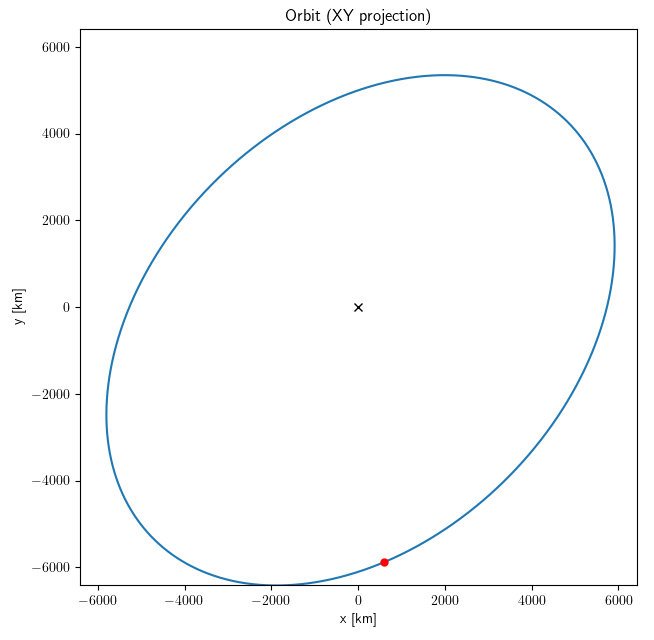
\includegraphics[width=\linewidth]{./outputs/figures/s04a1.png}
			\end{center}
			\caption{Orbit Plot 2D}
		\end{subfigure}
		\begin{subfigure}{0.5\textwidth} \label{fig:s04a2}
			\begin{center}
				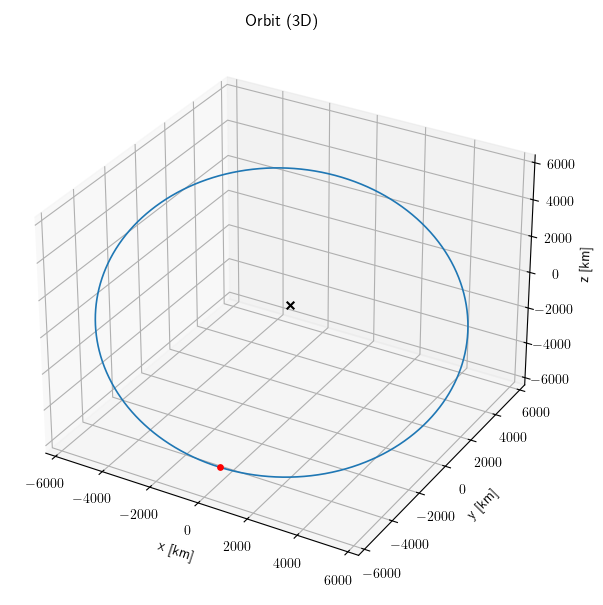
\includegraphics[width=\linewidth]{./outputs/figures/s04a2.png}
			\end{center}
			\caption{Orbit Plot 3D}
		\end{subfigure}
	\end{figure}

	\pagebreak

	\hwkPart{} \label{hwk:s04b}

	\begin{figure}[H] \label{fig:s04b}
		\begin{center}
			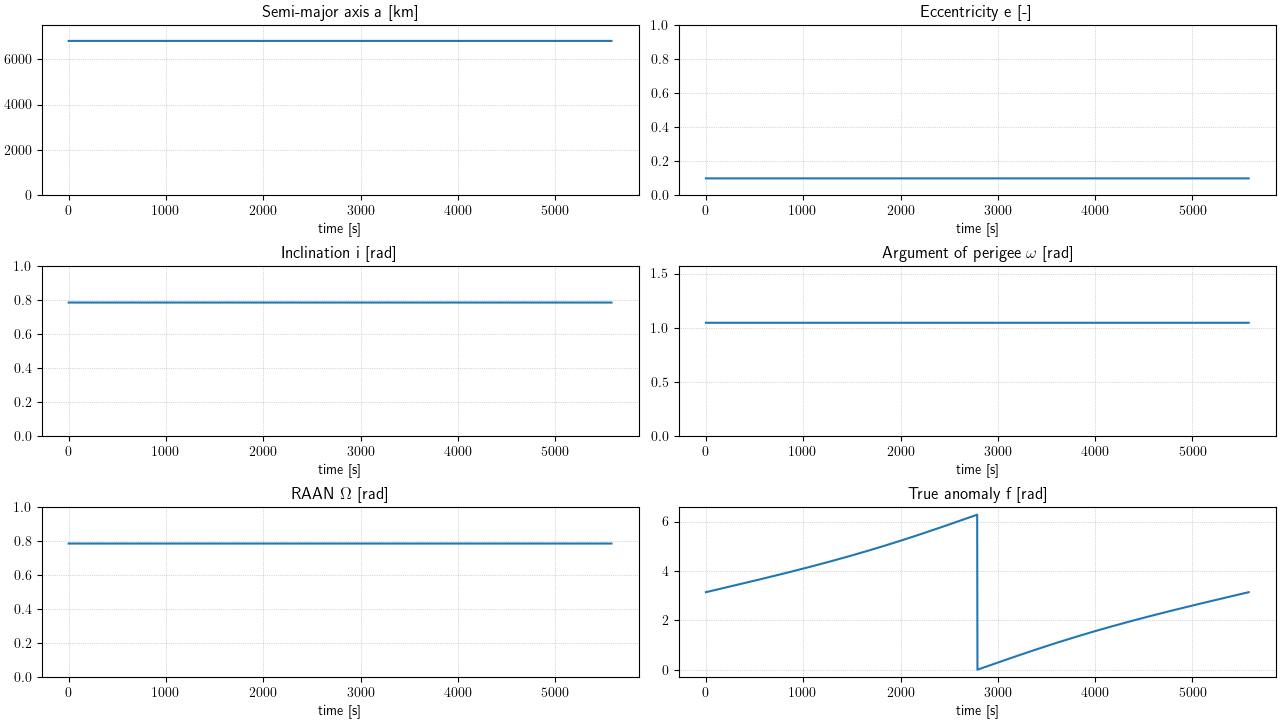
\includegraphics[width=0.9\linewidth]{./outputs/figures/s04b.png}
		\end{center}
		\caption{Orbital Elements vs. Time}
	\end{figure}

	\hwkPart{} \label{hwk:s04c}

	Due to being a pure two-body point-mass model (with no external forces nor third-body effects), the orbital plots depict a closed elliptical path, with perfectly repeated motion. A closed elliptical path should depict constant orbital elements \( a, e, i, \omega, \Omega \) — which we see in their respective orbital element plots. Such motion should also have steady procession in f wrt. time: beginning at \( f = f_{0} \), wrapping at \( f = 2 \pi \), and continuing its procession until \( f = f_{0} \) again — which we also see in its respective orbital element plot. Thus, all depicted behavior in the plots makes sense, as they line up with the expected behavior for a pure two-body system.

	\hwkCode{} \label{code:s04}

	See the \href{https://www.github.com/vaisriv/enae441-hw01/blob/main/src/hw01.py}{Python code} for this assignment.

\end{hwkProblem}

\end{document}
